
%------------------------------------------------
\begin{frame}
\frametitle{Metacognitive Exercises}
\note{\begin{itemize}
\item Pass out the printed Exercise number 1.
\item  The goal is to do the exercise fast and exact. 
\item Repeat one exercise with a new sheet for 20-21 days, before you start the next one. 
\item Write the date and the time needed on the paper to track your progress.
\end{itemize}
}


Developed by my teacher, Kilian Schmidt.


Metacognitive - \structure{transformational} for the \structure{intellect}, the
psyche, or \structure{thinking capacity}; and promotes development of
functions which contribute to perception or knowledge.

\begin{columns}[c] % The "c" option specifies centered vertical alignment while the "t" option is used for top vertical alignment

\column{.7\textwidth} % Left column and width
\begin{figure}
%
\includegraphics[width=1\linewidth]{Learning.jpg}
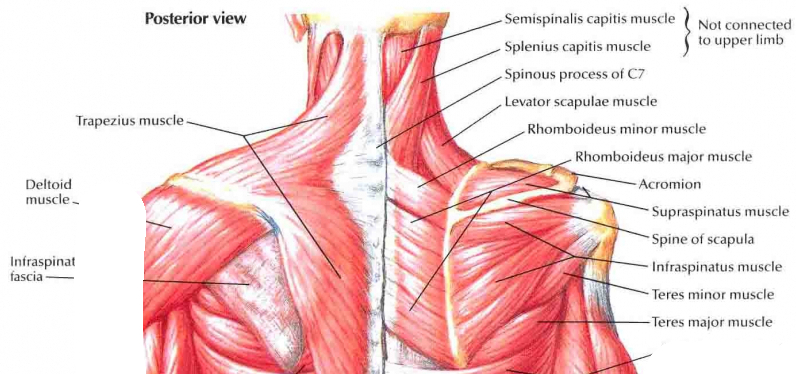
\includegraphics[width=\linewidth]{shoulder-muscles.jpg}
\end{figure}
\column{.38\textwidth} % Left column and width
\pause

Intention --- to \structure{influence the mental functions} with corresponding \structure{movements of our hand}.

Keep the arm above the writing surface. \note<2->{One of the most important indication muscles is then capable of  sending position signals to and training our brain in a positive way.}
\end{columns}

\end{frame}
%------------------------------------------------
%------------------------------------------------
\begin{frame}
\frametitle{Metacognitive Exercises: Effects}
\begin{columns}[c] % The "c" option specifies centered vertical alignment while the "t" option is used for top vertical alignment

\column{.5\textwidth} % Left column and width

%
\includegraphics[width=1\linewidth]{Learning.jpg}
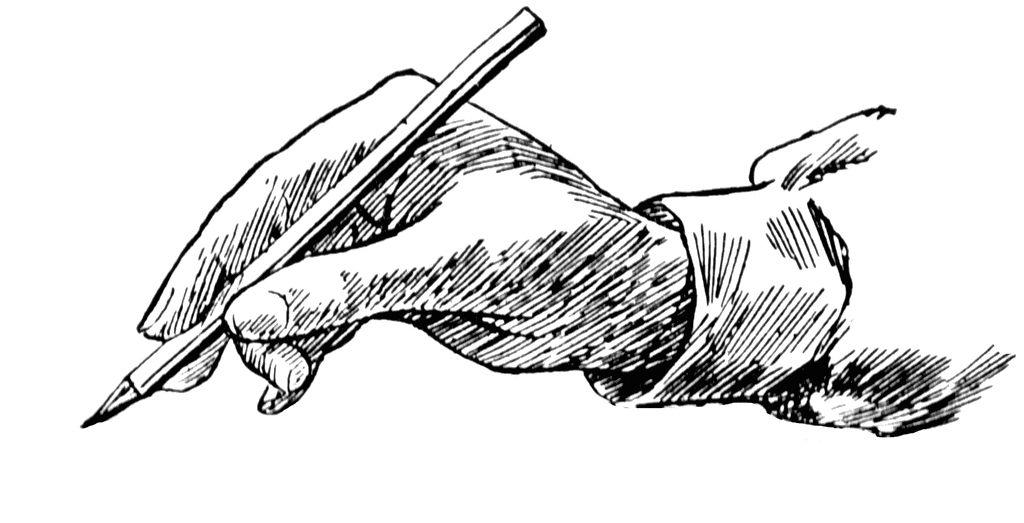
\includegraphics[width=\linewidth]{hw.jpg}



\column{.6\textwidth} % Left column and width

\pause
\begin{itemize}
\item[-] Improve the capacity to \structure{focus}.
\item[-]  Improves the quality of the \structure{awake state} for the whole day.
\item[-] Helps with \structure{thinking speed and endurance}.
\item[-] After practice, there may be improvement in \structure{stress dominant traits} (ie. test anxiety, low self--esteem and impaired problem--thinking).
\end{itemize}
\end{columns}
\note{Metacognitive exercises are often a way to get through a \structure{viscous circle}. 

A viscous circle is an unhindered dynamic. \structure{Obstructions}, coming from negative or sometimes even unreal thinking structures of the affected people, including excuses. The \emph{inner will to change} is missing.}

\vspace{1cm}
\href{run:./Metacognitive_Exercises.pdf}{\underline{Practice Sheets}}, 
or back to \href{run:./Exercises.pdf}{\underline{exercises}}.
\end{frame}
%------------------------------------------------
